% mycsrf 'for beeing included' snippet template
%
% (c) Karsten Reincke, Frankfurt a.M. 2012, ff.
%
% This text is licensed under the Creative Commons Attribution 3.0 Germany
% License (http://creativecommons.org/licenses/by/3.0/de/): Feel free to share
% (to copy, distribute and transmit) or to remix (to adapt) it, if you respect
% how you must attribute the work in the manner specified by the author(s):
% \newline
% In an internet based reuse please link the reused parts to mycsrf.fodina.de
% and mention the original author Karsten Reincke in a suitable manner. In a
% paper-like reuse please insert a short hint to mycsrf.fodina.de and to the
% original author, Karsten Reincke, into your preface. For normal quotations
% please use the scientific standard to cite
%

\section{w01: Easy\-ABC \ra\ abc2mtex \ra\ \LaTeX+Musix\TeX}\label{w01}

Entpackt man das Paket \texttt{abc2mtex1.6.1.tar.gz} aus dem genannten
Toolverzeichnis, kann man -- mit entsprechender Pfadangabe -- mittels
\texttt{\$PATH/abc2mtex} den Konverter mit der nativen ABC-Datei aufrufen, die
wir mit \acc{EasyABC} generiert und unter dem weg-spezifischen Subordner
\texttt{w01-easyabc-abc2mtex} abgelegt haben:


\begin{quote}\texttt{\$PATHX/abc2mtex \$PATHY/easyabc-cadenca3.abc}\end{quote}

Leider bricht das Programm mit einer Fehlermeldung ab:

\begin{quote}\texttt{error in input file easyabc-cadenca3.abc: line no. 10 - V
field not allowed in tune body }\end{quote}

Das ist 'leicht' erklärbar: Das ABC-Format war ursprünglich ein
Notationsverfahren für einstimmige 'Lieder'.\footnote{\ra\ S. \pageref{ABCMethod}}
Es ist erst später zu einem 'patitur-fähigen' Format erweitert worden. Der
Konverter \acc{abc2mtex} versteht nun offensichtlich nur das alte Format.
 
Daraus folgt nun leider, dass uns offensichtlich kein Verfahren zur Verfügung
steht, um Notentexte im \acc{Music\TeX}-Format über ein (semi-) graphischs
Frontend zu erfassen, und zwar auch dann nicht, wenn das Zielformat erst über
einen Konverter erzeugt werden darf.

\section{w02/w03: Easy\-ABC \ra\ abc2ly  \ra\ Frescobaldi/Elysium \ra\ \ldots}\label{w0203}

In dem weg-spezifischen Subordner \texttt{w02w03-easyabc-abc2ly} haben wir dieselbe
Ausgangsdatei \texttt{easyabc-cadenca3.abc} abgelegt, wie wir sie in und mit
\acc{EasyABC} generiert hatten:

\begin{center}
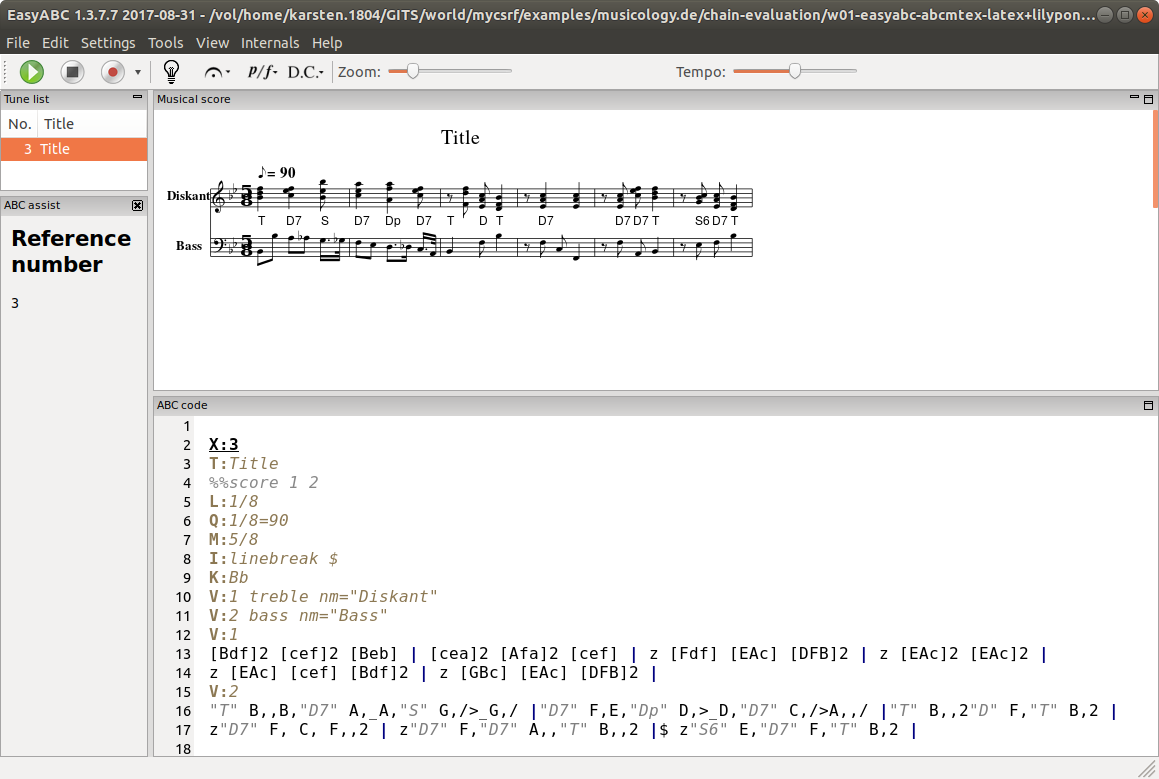
\includegraphics[width=0.9\textwidth]{frontends/easyabc/easyabc-cadenca3.png}
\end{center}

Mit dem folgenden Befehl kann man diese \acc{ABC}-Outputdatei in eine
\acc{LilyPond}-Datei konvertieren:

\begin{quote}\texttt{abc2ly -o easyabc-cadenca3.ly easyabc-cadenca3.abc}\end{quote}

Betrachtet man das Ergebnis in Frescobaldi, sieht man, dass die Konvertierung
nur sehr bedingt funktioniert hat:

\begin{center}
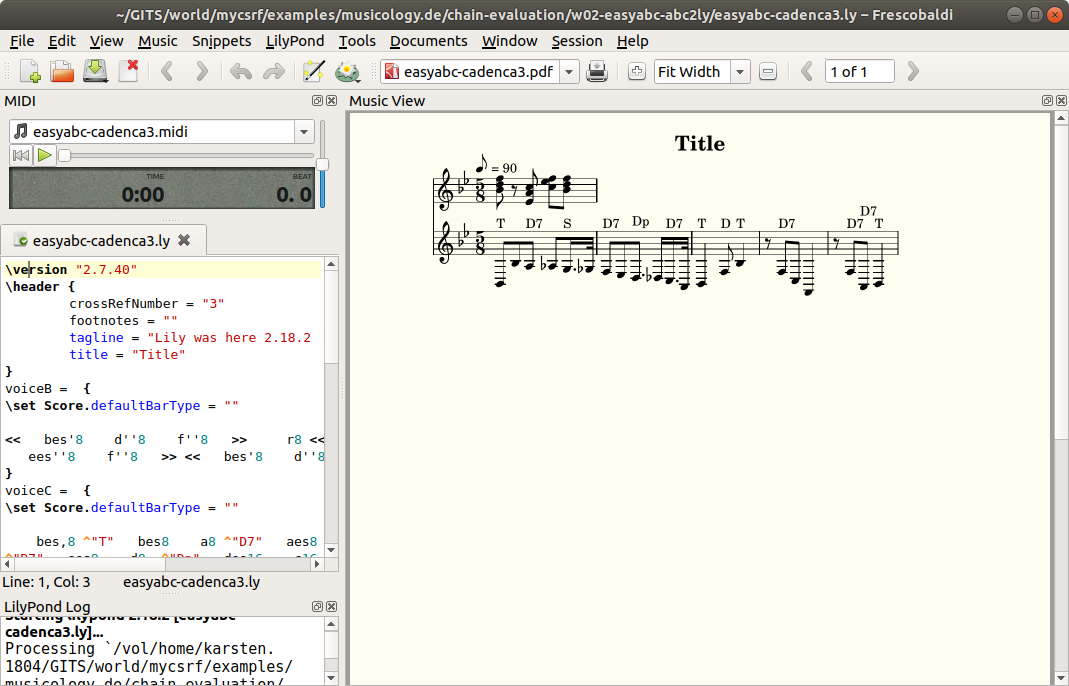
\includegraphics[width=0.9\textwidth]{frontends/easyabc/easyabc-cadenca3-abc-in-frescobaldi.png}
\end{center}

Daran ändert sich auch nichts, wenn man aus der \acc{EasyABC} die 'Texte'
entfernt und nur die Noten erfasst. 

\section{w04/w05: Easy\-ABC \ra\ musicxml2ly  \ra\ Frescobaldi/Elysium \ra\ \ldots}\label{w0405}

\acc{EasyABC} erlaubt es nicht nur, seine Daten im \acc{ABC}-Format zu
speichern, sondern auch, sie als \acc{Musicxml}-Datei zu exportieren. Damit wäre
zu überprüfen, ob der von \acc{LilyPond}-Konverter \acc{musicxml2ly} die
angelegten Daten so umformt, dass sie das erwartete Ergebnis in
\acc{Frescobaldi} und \acc{Elysium} bzw. \acc{LilyPond} generieren. Dazu haben
wir im weg-spezifischen Subordner \texttt{w04w05-easyabc-musicxml2ly} -- neben der
bisher schon genutzten Ausgangsdatei \texttt{easyabc-cadenca3.abc} -- auch die
Exportdatei \texttt{easyabc-cadenca3.xml} abgelegt. Daraus erzeugt man mit
folgendem Befehl die entsprechende \acc{LilyPond}-Datei generieren:

\begin{quote}\texttt{musicxml2ly easyabc-cadenca3.abc}\end{quote}

Und wenn man diese Datei mit \acc{Frescobaldi} öffnet, erhält man eine perfekte
Umformung:

\begin{center}
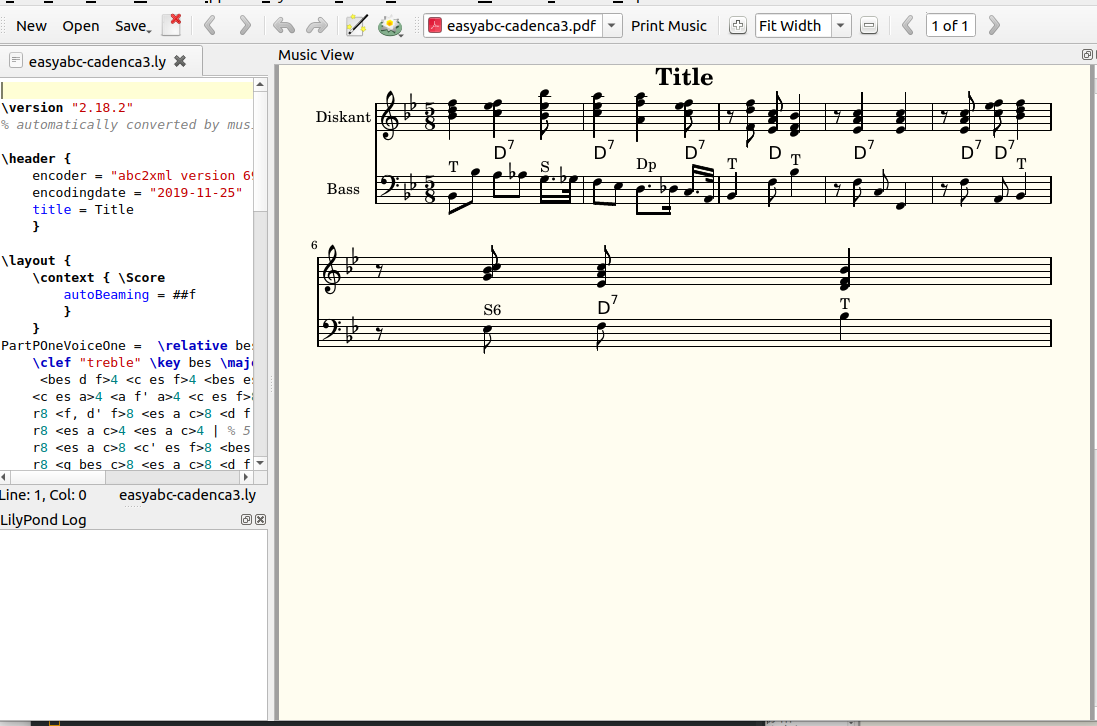
\includegraphics[width=0.9\textwidth]{frontends/easyabc/easyabc-musicxml-frescobaldi.png}
\end{center}

\section{w06/07: Muse\-Score \ra\ musicxml2ly \ra\ Frescobaldi / Elysium \ra\ \ldots}\label{w0607}

Schließlich haben wir in dem Ordner
\texttt{[\ldots]/musicology/chain-evaluation/} den weg-spezifischen Subordner
\texttt{w0607-musescore-musicxml2ly} erzeugt und darin die Kandenz-III als
\acc{MuseScore}-Datei (\texttt{cadenca3.mscz}) und den korrespondierenden
MusicXML-Output (\texttt{cadenca3.xml})abgelegt:

\begin{center}
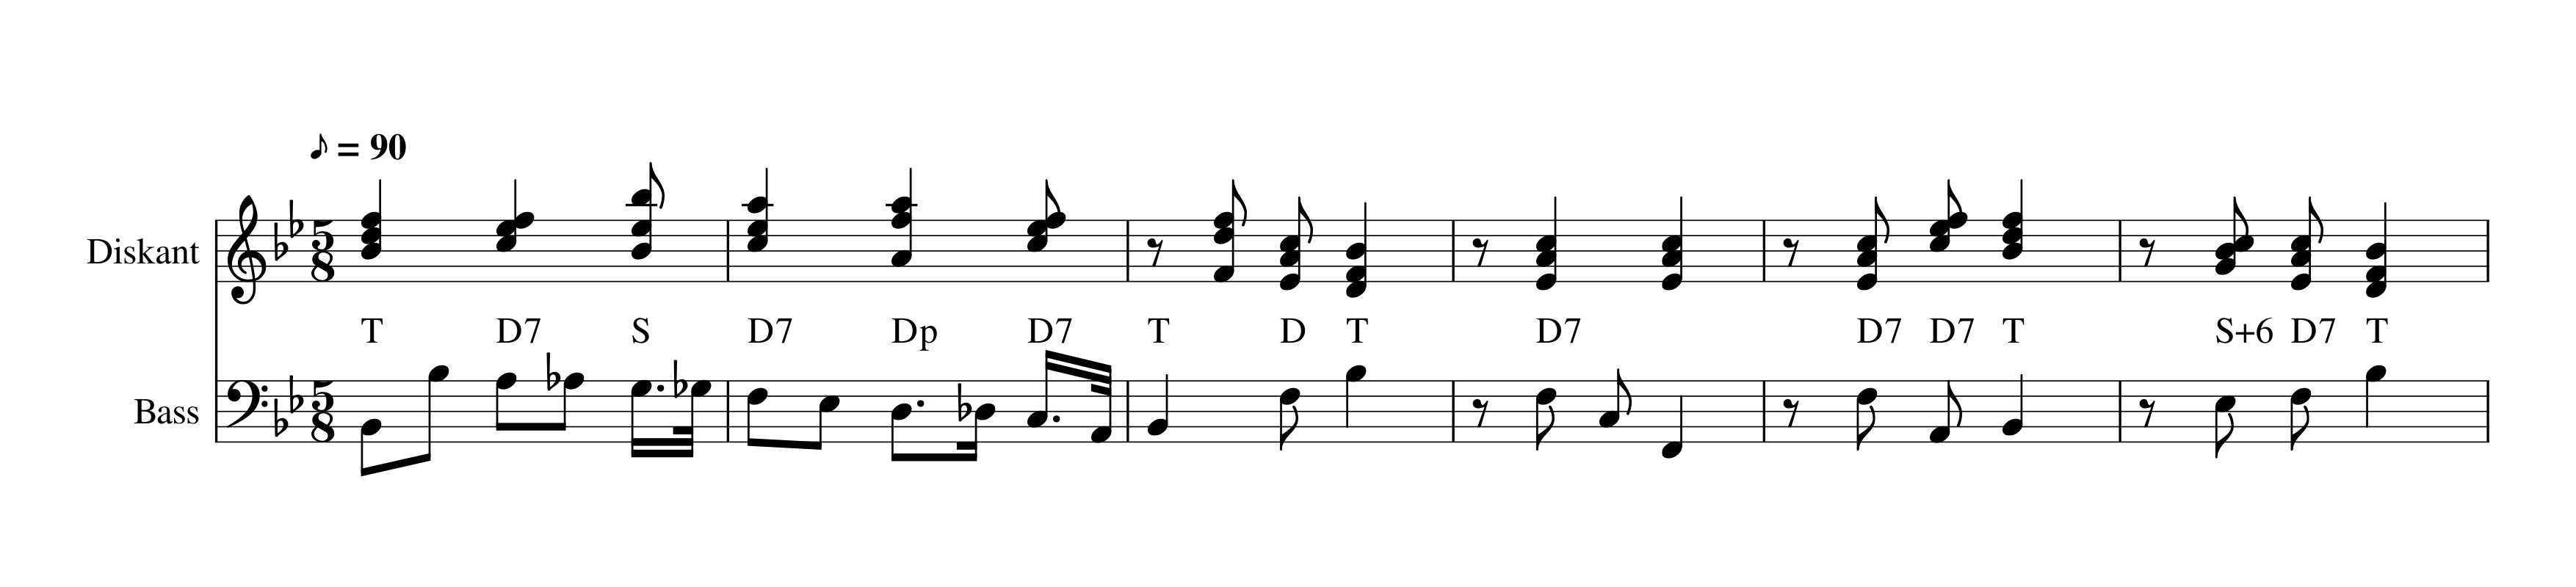
\includegraphics[width=0.9\textwidth]{frontends/musescore/cadenca3-musescore-300dpi.png}
\end{center}

Damit sollte sich auch die XML-Datei in eine \acc{LilyPond}-Datei konvertieren lassen:

\begin{quote}\texttt{musicxml2ly -o cadenca3.ly cadenca3.xml}\end{quote}

Technisch läuft die Konvertierung problemlos durch. Das Ergebnis sieht in
\acc{Frescobaldi} nicht so schlecht aus:


\begin{center}
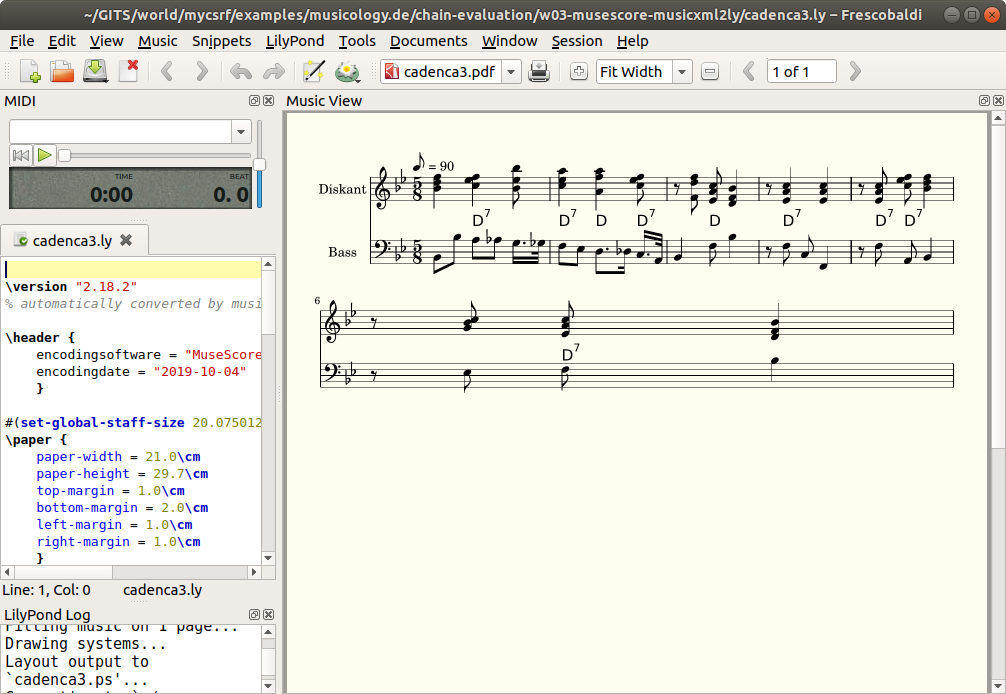
\includegraphics[width=0.9\textwidth]{frontends/musescore/musescore-cadenca3-in-frescobaldi.png}
\end{center}

Einzig sind einige Harmoniesymbole unter den Tisch gefallen, die eh durch die
äquivalenten Ausdrücke über unser Zusatzbibliothek \acc{harmonyli} ersetzt
werden sollen.

Damit dürfen wir sagen, dass man \acc{LilyPond} auch mit einem echten
graphischen Frontend verwenden kann, nämlich mit \acc{MuseScore}, sofern man
auch den von \acc{LilyPond} gepflegten Konverter \acc{musicxml2ly}
verwendet. Dass das Frontend \acc{MuseScore} von sich aus keine adäquaten
Harmonieanalysesymbole mitbringt, ist kein Nachteil: man lässt sie ja eh
weg, um später über die semi-graphische Editoren \acc{Frescobaldi} oder
\acc{Elysium} die Syntagmen nachzutragen, die die Bibliothek \acc{harmonyli.ly}
in die Gesatltung einbringt.


\section{Vergleich}

So können wir die Ergebnisse in Sachen einer Verknüpfung von Frontend und Backend
zusammentragen:

\begin{footnotesize}

\begin{tabular}{|c||c|c|c|c|c||c||}

% was soll am Anfang oben scheinen:
\hline
  \multirow{2}{*}{\rotatebox{90}{Weg\ }} & \multicolumn{2}{c}{VON} & \multicolumn{1}{|c}{ÜBER} & 
  \multicolumn{2}{|c||}{NACH} & = \\
\cline{2-7}
 & Frontend & $\bigstar$ & Konvertierung & \LaTeX\ + & $\bigstar$ & \\
\hline
\hline
01 & EasyABC & 4 & \ra\ abc2mtex \ra\ & Musix\TeX\ & 4 &  \texttt{-} \\
\hline
02/03 & EasyABC & 4 & \ra abc2ly \ra\ Frescobaldi/Elysium \ra\ & LilyPond & 5 &  \texttt{-} \\
\hline
04/05 & EasyABC & 4 & \ra musicxml2ly \ra\ Frescobaldi/Elysium \ra\ & LilyPond & 5 &  \texttt{++} \\
\hline
06/07 &  MuseScore & 5 & \ra musicxml2ly \ra\ Frescobaldi/Elysium \ra\ & LilyPond & 5 & \texttt{++} \\
\hline
08 &  Frescobaldi & 5 & \ra\ & LilyPond & 5 & \texttt{++}  \\
\hline
09 & Elysium & 4 & \ra\ & LilyPond & 5 & \texttt{++}  \\
\hline
\hline
\end{tabular}
\end{footnotesize}

Und damit reduziert sich unsere Wegskizze noch einmal:

\begin{tikzpicture}
\footnotesize

\tikzstyle{every node}=[trapezium, draw, minimum width=1cm,trapezium left angle=70, trapezium right angle=110]

% BOTTOM UP DESCRIPTION of the component IO structure:
% THE FINALLY GENERATED PDF OUTPOUT ->
\file{\pdfBgColor}{black}{PDF}{5.5}{0}{.pdf}

% -> CREATED BY THE LATEX IDEs ->
\backend{$\star\star\star\star$}{\mtexColor}{LTXMTEX}{5.5}{2}{\LaTeX\,+\,MusiX\TeX}
\backend{$\star\star\star\star\star$}{\lyColor}{LTXLIPO}{10.4}{2}{\LaTeX\,+\,LilyPond}

% -> which take the CONVERTER OUTPUT ->
\file{\mtexBgColor}{\mtexColor}{CO-MTEX}{5.5}{3}{.mtex}
\file{\lyBgColor}{Blue}{CO-LY}{10.4}{3}{.ly}

% written by the CONVERTERs.

\converter{\mxmlInColor}{\lyOutColor}{MUSICXML2LY}{4.8}{8.8}{musicxml2ly}



% These converters takte the FRONTEND OUTPUT ->


\file{\mxmlBgColor}{\mxmlColor}{FO-MXML}{1.5}{10}{.mxml}
\file{\lyBgColor}{Blue}{FO-LY}{7}{8.8}{.ly}

% created by the FRONTENDS ->

\frontend{\abcBgColor}{Black}{EASYABC}{0}{12.5}{EasyABC}{$\star\star\star\star$};
\frontend{\multiBgColor}{Black}{MUSESCORE}{4.5}{13.5}{MuseScore}{$\star\star\star\star\star$};

\frontend{\multiBgColor}{Black}{EDITOR}{7.7}{7.2}{Text-Editor}{$\star$};
\frontend{\lyBgColor}{Black}{ELYSIUM}{9.8}{6.8}{Elysium}{$\star\star\star\star$};
\frontend{\lyBgColor}{Black}{FRESCOBALDI}{11.9}{6}{Frescobaldi}{$\star\star\star\star\star$};

% which are used by the Composer:

%
\node[rectangle, draw=none, inner sep=0pt] (Composer) at (8.3,15.5) 
{
\includegraphics{./logos/decider-220x320.eps}};
  
% TOP DOWN linkings of the component IO structure:  
  
% (1) The composer uses the frontends.
\draw[->] (Composer) to [out=180,in=70] (EASYABC);  
\draw[->] (Composer) to [out=180,in=70] (MUSESCORE);   
\draw[->] (Composer) to [out=0,in=90] (ELYSIUM);  
\draw[->] (Composer) to [out=0,in=90] (FRESCOBALDI);  
\draw[->] (Composer) to [out=0,in=90] (EDITOR);  

 
% (2.A) The frontends write the frontend output  

\draw[->,\mxmlColor] (EASYABC) to [out=300,in=90] (FO-MXML); 
\draw[->,\mxmlColor] (MUSESCORE) to [out=240,in=90] (FO-MXML); 
\draw[->,\mtexColor] (EDITOR) to [out=270,in=0] (CO-MTEX);
\draw[->,\lyColor] (ELYSIUM) to [out=270,in=90] (CO-LY); 
\draw[->,\lyColor] (FRESCOBALDI) to [out=270,in=90] (CO-LY); 

% (3) The frontend output becomes input of the converter

\draw[->,\mxmlColor] (FO-MXML) to [out=270,in=90] (MUSICXML2LY);


%\draw[->,\lyColor] (FO-LY) to [out=270,in=90] (LY2ABC); 
%\draw[->,\lyColor] (FO-LY) to [out=270,in=90] (EDITOR); 
\draw[->,\lyColor] (FO-LY) to [out=360,in=90] (ELYSIUM); 
\draw[->,\lyColor] (FO-LY) to [out=360,in=90] (FRESCOBALDI); 

% (3) The converters (re)write their output
% (3.A) as input for the textual frontends
\draw[->,\lyColor] (MUSICXML2LY) to [out=0,in=180] (FO-LY); 

% (3.B) as input for the backends

% 4) The backends take the (converter) output as input
\draw[->,\mtexColor] (CO-MTEX) to [out=270,in=90] (LTXMTEX);
\draw[->,\lyColor] (CO-LY) to [out=270,in=90] (LTXLIPO);

% 5) end write the final PDF
\draw[->,Black] (LTXMTEX) to [out=270,in=90] (PDF);
\draw[->,Black] (LTXLIPO) to [out=270,in=90] (PDF);
\end{tikzpicture}